%=============================================================================
% CHAPTER 1: INTRODUCTION
%=============================================================================

\chapter{Introduction}

\section{Background and Motivation}

In the digital age, passwords remain the most common and accessible method people use to secure online accounts and protect sensitive information. Despite their widespread use, weak and reused passwords continue to represent one of the leading vulnerabilities exploited in modern cybersecurity incidents. Even with technological advances in authentication methods, such as biometrics, hardware tokens, or two-factor/multi-factor verification, the vast majority of online services still rely on traditional passwords as the first line of defence.

During my studies and everyday use of technology, I noticed that most users tend to underestimate the importance of password strength and good password hygiene. Many choose simple or predictable combinations such as ``123456'' or ``password,'' unaware that such passwords can be guessed in seconds by automated tools using dictionary attacks, brute-force techniques, or credential stuffing. In addition, users frequently reuse the same password across multiple platforms, meaning that a compromise of a single account can easily cascade into a much larger security incident. This widespread lack of awareness, combined with poor password management habits, contributes significantly to the increasing number of successful data breaches, identity thefts, and unauthorised account takeovers.

According to the Verizon Data Breach Investigations Report, approximately 80\% of hacking-related breaches involve compromised or weak credentials \cite{verizon2024}. The NordPass annual report on the most common passwords consistently shows that trivially guessable passwords such as ``123456,'' ``admin,'' and ``password'' dominate the top positions year after year \cite{nordpass2024}. These statistics underscore the persistent gap between the known best practices and the actual behaviour of everyday users.

\begin{figure}[H]
    \centering
    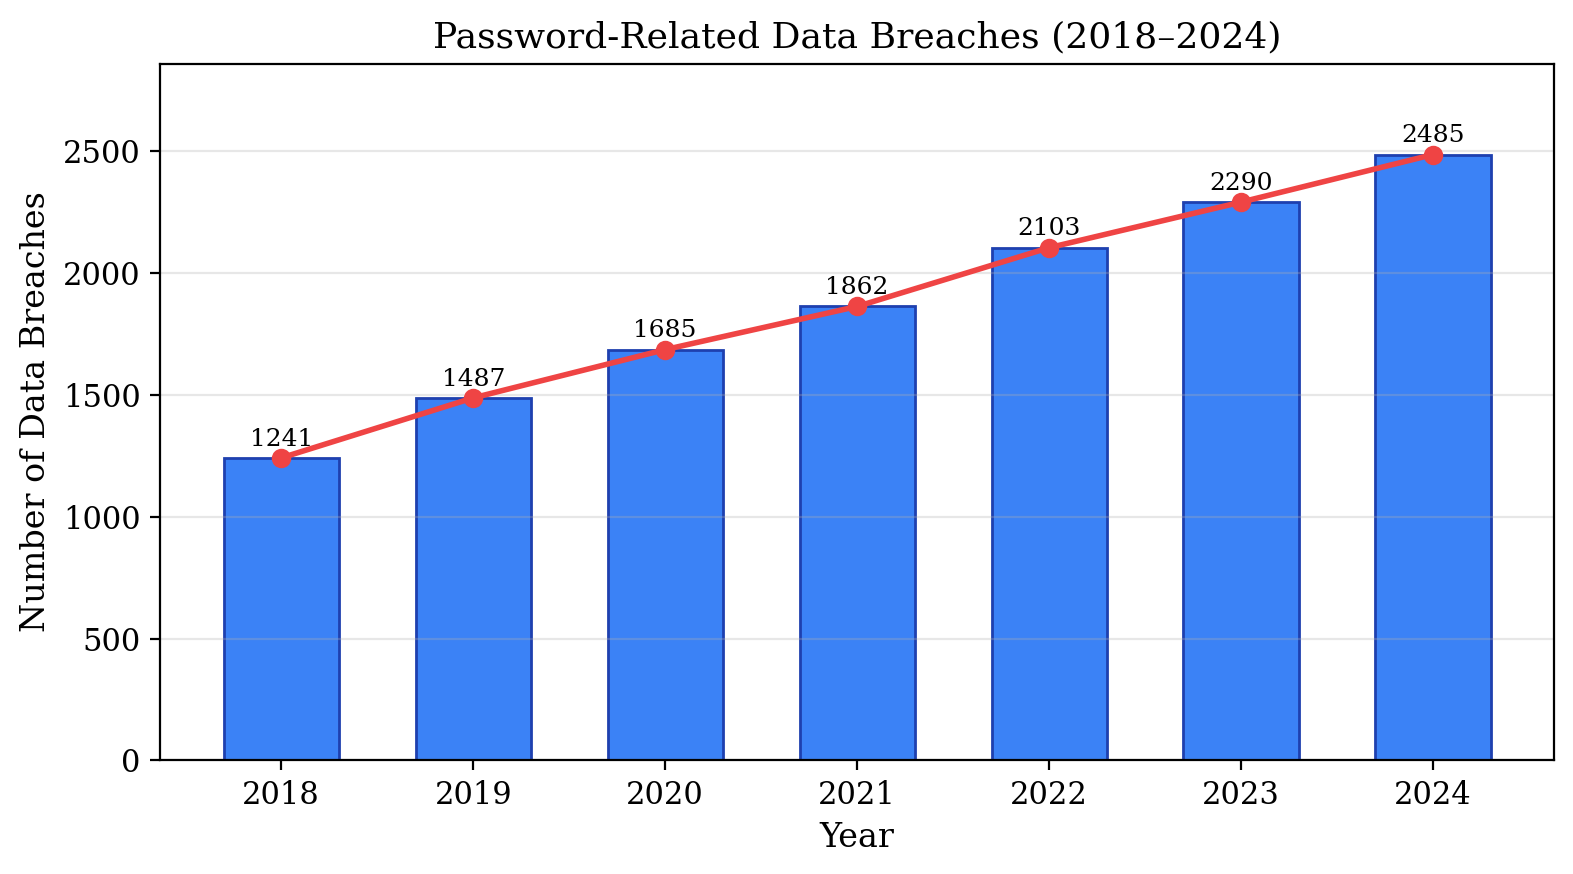
\includegraphics[width=0.85\textwidth]{figures/password_breach_trend.png}
    \caption{Trend of password-related data breaches from 2018 to 2024.}
    \label{fig:breach_trend}
\end{figure}

\begin{figure}[H]
    \centering
    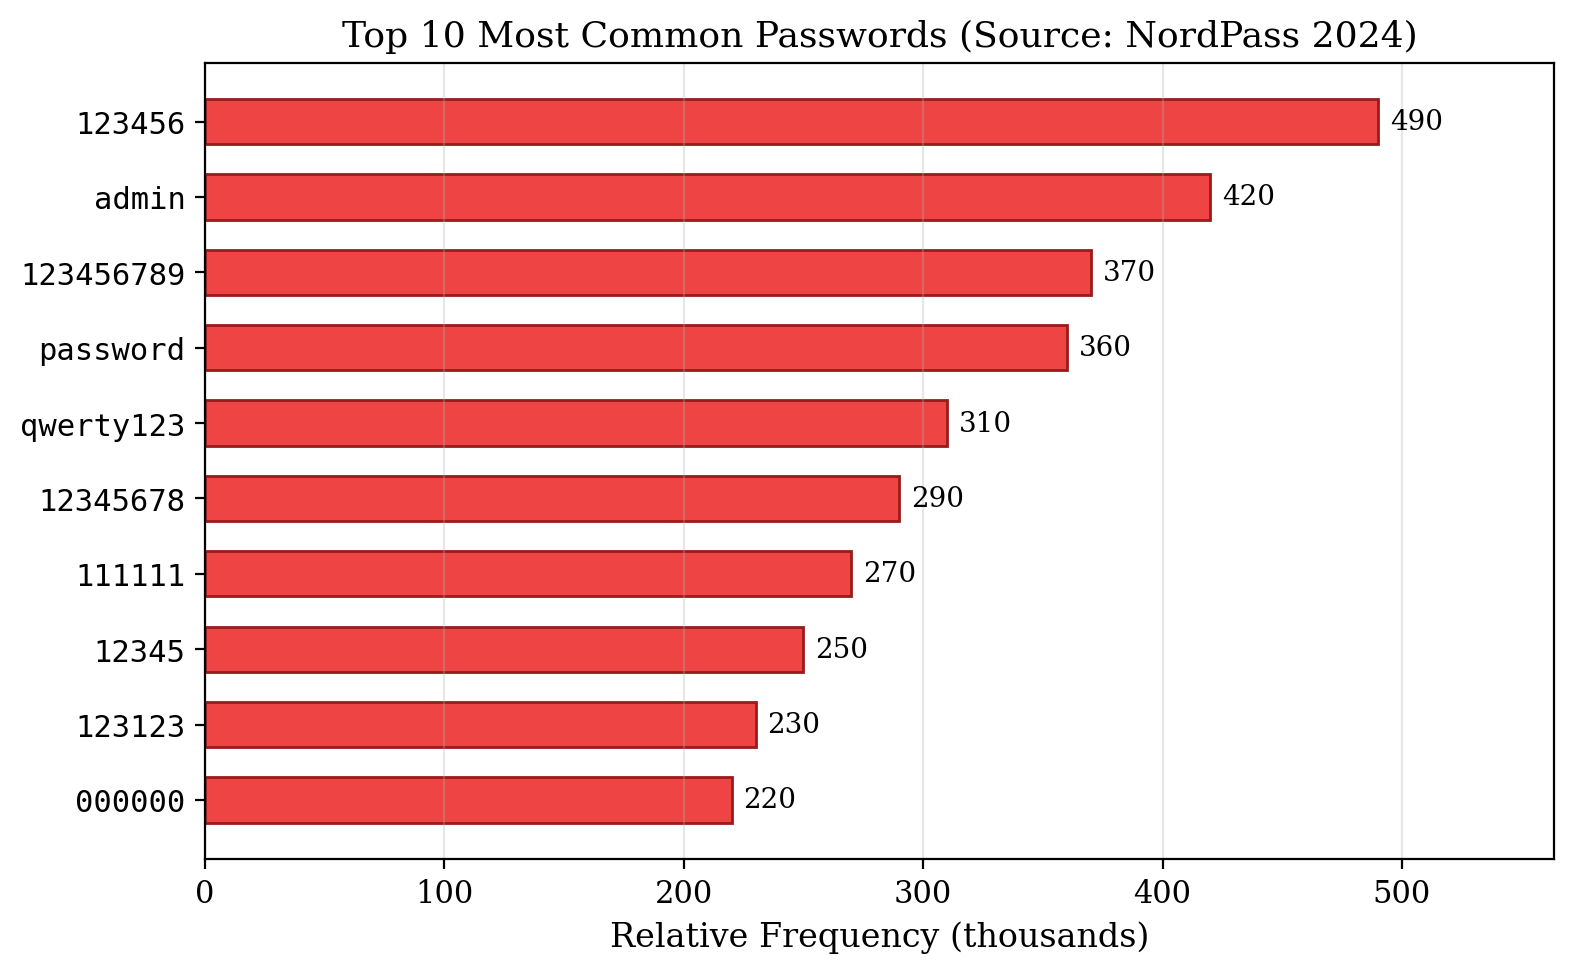
\includegraphics[width=0.85\textwidth]{figures/top_passwords_chart.png}
    \caption{Top 10 most common passwords and their usage frequency.}
    \label{fig:top_passwords}
\end{figure}

I have always been interested in practical applications of cybersecurity, especially in areas where user behaviour directly affects digital safety. For that reason, I decided to develop a password strength evaluation tool that helps users understand how secure their passwords are and how to improve them. The tool aims not only to give a numerical or qualitative strength rating, but also to provide clear, actionable feedback on issues such as length, character diversity, resistance to common attack patterns, and susceptibility to known leaked-password lists.

The project combines both theoretical knowledge about password security—such as entropy, common attack vectors, and best-practice guidelines from standards like NIST— with the practical skills I have gained in Python programming, including modular software architecture, secure handling of user data, graphical interface design, and implementation of hybrid security checks. Through this work, I aim to raise awareness of secure password practices and contribute to a safer online experience for everyday users.


\section{Aim of the Thesis}

The main aim of my thesis is to design, implement, and evaluate a Python-based desktop application with a graphical user interface and real-time hybrid analysis that can assess the strength of user passwords and provide constructive, user-friendly feedback. Through this project, I intend to demonstrate my ability to analyse a real-world cybersecurity problem, design an algorithmic solution based on established security principles and current best practices, and implement it as a functional, maintainable, and extensible tool that can be realistically deployed in contemporary computing environments.

Specifically, the objectives of the thesis are to:
\begin{itemize}
    \item analyse common patterns and weaknesses that make passwords insecure, including predictable structures, reuse of credentials across multiple services, use of personal or easily guessable information, and susceptibility to automated attacks,
    \item develop a hybrid algorithm that assesses password strength based on five measurable dimensions---length, character diversity, entropy, pattern detection, and dictionary comparison---while keeping the model transparent and interpretable to end users through named scoring constants and clear feedback,
    \item identify dictionary words and common patterns (such as keyboard sequences, reversed keyboard patterns, repeated or sequential characters, leetspeak variants, and predictable substitutions) that lower security, and incorporate these findings into the scoring and feedback mechanism,
    \item design a dark-themed graphical user interface with CustomTkinter that provides real-time password analysis through a debounced input mechanism, animated visual indicators, and a two-column analysis layout that presents both a score overview and detailed improvement suggestions simultaneously,
    \item implement an iterative improvement process, documented through 18 systematic enhancements and a user-experience redesign, demonstrating that structured quality refinement leads to a measurably better tool,
    \item generate meaningful, context-aware feedback to help users create stronger passwords by suggesting specific improvements and explaining the underlying security rationale in clear, non-technical language, with suggestions originating from the evaluation engine to ensure a single source of truth,
    \item validate the effectiveness, robustness, and usability of the proposed evaluation method through functional testing on representative password samples, comparative analysis with existing password-strength meters, and a usability self-evaluation based on Nielsen's heuristics,
    \item document design decisions, limitations, and potential security and privacy concerns (such as safe handling of input passwords) to inform future extensions and responsible use of the tool.
\end{itemize}

The purpose of the system is educational as well as practical---to raise user awareness of password security through an easy-to-use, self-contained tool that can be integrated into introductory cybersecurity training, personal use, or small-scale organisational environments. In addition, the system is intended to serve as a reference implementation that can be adapted or extended in future work, for example by incorporating machine-learning-based estimators, support for passphrases, or integration into web and mobile authentication workflows.


\section{Scope of the Thesis}

The thesis comprises both a theoretical and a practical component. The theoretical part examines the foundations of password security, including threat models, common attack methods (such as brute-force, dictionary, and credential-stuffing attacks), and the mathematical concepts used to measure password robustness, such as entropy, search space, and estimated attack complexity. It also reviews existing password-strength evaluation approaches and guidelines from recognised standards (e.g.\ NIST recommendations and relevant industry best practices) to situate the proposed tool within the broader context of password security research and practice. Where appropriate, the limitations and known shortcomings of current approaches are discussed in order to motivate specific design choices made in this work.

The practical part focuses on the development process of the proposed tool, including requirements analysis, modular architectural and interface design decisions, algorithm implementation, and both functional and non-functional testing, followed by a systematic evaluation. The implementation is built as a Python desktop application using CustomTkinter for the graphical user interface, featuring a dark-themed dashboard with real-time analysis via a 300\,ms debounced input mechanism, a two-column analysis layout, animated semicircular gauge and horizontal meter bar, and a cryptographically secure password generator. Particular attention is paid to code quality, modularity, performance, and maintainability, as well as the ease with which the tool can be adapted or extended (for example, to new dictionaries, language-specific patterns, or additional attack models). The development followed an iterative process of 18 systematic enhancements and a user-experience redesign, which is documented in detail.

I deliberately limit the project's scope to password strength evaluation and do not address topics such as encryption algorithms, password storage mechanisms (e.g.\ hashing and salting), multi-factor authentication, federated identity management, or large-scale authentication infrastructures. These subjects are important and closely related areas of cybersecurity but fall beyond the intended scope of a first-cycle practical project and would require separate, dedicated treatment and substantially broader technical coverage.

\clearpage

\section{Justification of the Topic Choice}

I chose this topic because it allows me to apply theoretical cybersecurity knowledge in a way that produces a tangible, working result. The password strength evaluator represents a concrete example of how programming and security theory can directly contribute to improving digital safety in everyday scenarios. It also enables me to demonstrate key skills---problem analysis, requirements engineering, algorithmic design, software implementation, documentation, and empirical evaluation---all of which are crucial in my field of study and highly valued in professional practice.

Moreover, the topic remains highly relevant. Data breaches caused or facilitated by weak, reused, or predictable passwords continue to occur regularly, affecting both individuals and organisations across different sectors \cite{verizon2024}. Despite the availability of advanced authentication methods (such as hardware tokens and biometric systems), passwords remain the dominant mechanism for user authentication on most systems and services. Accessible tools that educate users, help them understand the limitations of their current password choices, and encourage better practices are therefore needed more than ever.

\subsection{Contribution to Society}

Beyond personal skill development, this project addresses a genuine societal problem: the persistent gap between cybersecurity best practices and everyday user behaviour. The tool contributes to society in several concrete ways:

\begin{itemize}
    \item \textbf{Increasing user awareness:} By providing immediate, context-aware feedback as users type their passwords, the tool educates them about the specific weaknesses in their choices. Each suggestion explains not only \textit{what} to change but also \textit{why}---for example, ``Avoid keyboard patterns like qwerty or asdf---these are in every cracking dictionary.'' This educational approach helps users internalise good password practices rather than merely following rules mechanically.

    \item \textbf{Preventing common attacks through education:} The tool's hybrid evaluation model explicitly addresses the three most common password attack strategies---brute-force (through length and entropy scoring), dictionary attacks (through dictionary comparison and Levenshtein similarity), and pattern-based attacks (through sequential, repeated, and keyboard pattern detection). By making users aware that these attack strategies exist and that their passwords are vulnerable to them, the tool encourages the creation of passwords that resist all three.

    \item \textbf{Promoting better password hygiene:} The actionable suggestions and the integrated ``Generate Strong Password'' feature encourage users to move beyond simple, reused passwords toward stronger, unique credentials. The real-time feedback loop---type, evaluate, improve, re-evaluate---makes the process of strengthening a password feel natural and achievable rather than burdensome.

    \item \textbf{Providing a privacy-friendly alternative:} Unlike most online password checkers, which require transmitting the password over the internet, this tool processes everything locally. No passwords are stored, logged, or transmitted at any point. This privacy-first design means that users can evaluate their most sensitive passwords without risking exposure to third-party services, a concern that has become increasingly important as data breaches continue to make headlines \cite{verizon2024}.

    \item \textbf{Democratising security knowledge:} The transparent scoring model, with its named constants and explainable breakdown, makes the evaluation process accessible to non-technical users. Unlike ``black box'' strength meters that provide a rating without explanation, this tool shows exactly how each dimension contributes to the final score, empowering users to make informed decisions about their password choices.
\end{itemize}

This project, while small in scale, aims to make a meaningful contribution to everyday cybersecurity awareness by providing a transparent, explainable password evaluation tool. The implementation emphasises interpretability, so that users not only receive a strength score but also understand the reasoning behind it and the specific changes that can improve their passwords. A distinctive contribution of this tool is its detection of reversed keyboard patterns---a weakness that most existing online password checkers fail to identify---demonstrating that even a compact, locally-run tool can offer analysis capabilities absent from some widely-used web-based checkers.

In addition to its immediate practical use, the tool can serve as a starting point for further work, such as integrating the evaluator into web applications, extending it to support multiple languages and cultural password patterns, combining it with password managers, or embedding it into broader security education initiatives and institutional security policies.

\clearpage

\section{Thesis Layout}

The structure of my thesis is organised as follows:
\begin{itemize}
    \item \textbf{Chapter 1} introduces the topic, defines the aim, scope, and motivation for the project.
    \item \textbf{Chapter 2} presents the theoretical background, including password vulnerabilities, mechanisms of password attacks, real-world breaches, entropy, existing evaluation techniques, and tools and standards.
    \item \textbf{Chapter 3} explains the methodology, system architecture, the hybrid evaluation algorithm, detection techniques, and the user interface approach.
    \item \textbf{Chapter 4} describes the implementation process, including project structure, the evaluation engine pipeline, core analysis modules, password generation, and the graphical interface.
    \item \textbf{Chapter 5} presents functional test results, a comparative analysis with existing tools, a usability self-evaluation, a discussion of advantages and disadvantages, and limitations.
    \item \textbf{Chapter 6} concludes the thesis with a summary of achievements, final conclusions, and possible future extensions.
\end{itemize}